\section{Navigation Test}

The robot must enter the arena, visit each one from a set of waypoints, and then follow a human outside the arena. After following, the robot must guide a human back to the arena. 
The path from a waypoint to another often blocked by an obstacle that requires the robot to take an action to solve the task.

Actions may include: avoid the obstacle, find a different path, or even interact with the obstacle (move it, open it, ask it to move, wait for it to move, etc.).

\subsection{Goal}
This test is about dealing with obstacles and navigating with a human companion. 
The robot must be able navigate through the apartment, avoiding or interacting obstacles along the way.
After that, the robot must demonstrate its ability to follow someone and the ability to guide someone. 

\subsection{Focus}
The navigation test focuses on navigating in a changing environment, where doors can be closed and even paths to goal may get blocked by movable temporary objects.
Perceiving the obstacles is also critical in safely navigating a home environment.

For a care environment, the ability to follow and guide a human are also important. 

\subsection{Setup}

\begin{enumerate}
	\item \textbf{Location:} One of the arenas (apartment). The apartment is in its normal state.
	\item \textbf{Doors:} All doors in the apartment are open, except for the entry door. 
	The arena will likely contain another door that may be used for this test. 
\end{enumerate}

\subsection{Task}
The robot must visit a set of waypoints and avoid the obstacles on its path. Unless stated otherwise, waypoints may be rooms, placement locations, furniture, beacons or landmarks on the floor. 
The robot must state when it reached a new waypoint or is not able to reach a waypoint. 
At the last waypoint inside the arena, the robot must follow a human which will lead the robot outside. 
After the robot is commanded to stop following, the robot must guide a (different) human back to the apartment. 

\begin{enumerate}
	\item \textbf{Entering the arena:} The robot starts outside the environment and must wait until the door opens.

	\item \textbf{Waypoint 1 (door):} After entering the arena, the robot must navigate to \textit{Waypoint 1}, 
	  which may be any location and is reachable via several paths that may include one of more doors.
	One of the doors may be shut. The robot may:
	\begin{itemize}
		\item To take a different path.
		\item Open the closed door.
	\end{itemize}

	\item \textbf{Waypoint 2 (obstructed path):} After reaching \textit{Waypoint 1}, the robot must navigate and reach (to within grasp or place distance) 
	  \textit{Waypoint 2}, which is a placement location, e.g. a table. 
	However, some sort of obstacle is present at \textit{Waypoint 2} e.g. people or movable furniture (e.g.~ a wheelchair) with which the robot may interact in order to reach its destination. 
	The robot may:
	\begin{itemize}
		\item Move the obstacle (if the obstacle is an object).
		\item Ask the obstacle to move out (if the obstacle is a human).
		\item Wait for the object to move away by itself (if the obstacle is another robot).
		\item Take a different approach to the waypoint. E.g. if the obstacle is a table and one end is unreachable, go to the other end of the table). 
	\end{itemize}

	\item \textbf{Waypoint 3 (following a human):} After reaching \textit{Waypoint 2}, the robot must navigate to \textit{Waypoint 3}, a landmark or beacon. 
	Here will be waiting a \textit{Professional Walker} the robot must memorize and follow outside the arena.

	\begin{enumerate}
	\item \textbf{Memorizing the operator (training phase):} The robot has to memorize the operator.
	During this phase, the robot may instruct the operator to follow a certain setup procedure and instruct the operator on what to do when the robot needs to stop following.
	
	\item \textbf{Following the operator (guiding phase):} 
	When the robot signals that it is ready to start, the operator starts walking --in a natural way-- through a designated path outside the arena. 
	The robot needs to follow the operator until the operator asks the robot to stop doing so (\textit{Waypoint 4}).
	\end{enumerate}

	\item \textbf{Waypoint 4 (stop following):} Upon reaching \textit{Waypoint 4}, 
	  the \textit{Professional Walker} will command the robot to stop following him, using the instructions given by the robot in the training phase.
	
	\item \textbf{Optional: Guiding a human:} Then, the robot must guide a human back to the starting point (\textit{Waypoint 3}).
	The human will stand in front of the robot, which instructs the human on what to say to start the guideing. 
	After some time, the human gives the command to start the guiding (e.g. ``Take me to my appartment'').
	The robot must then go back to the starting point (\textit{Waypoint 3}), while checking that the human is still following and has not stopped or has drifted off on a different path.
	
	This implies the human is not touching the robot or vice versa. 
	
	\begin{itemize}
	 \item In case the human drifts off, the robot must stop and call the human back. 
% 	 \item In case the human drifts off, the robot must get the human, stand in front of him/her, call the human to attention and start guiding further.
	 \item The guide phase is about 10-20 meters.
	 \item Once back at \textit{Waypoint 3}, the robot must tell the human he/she is back home. 
	 \item Attempting the guide-phase gives an additional 5 minutes. 
	  The guide-phase must finish within 5 minutes. 
	\end{itemize}
	
	\item \textbf{Going back:} If the robot is unable to guide a human, it must go back to the starting point (\textit{Waypoint 3}) alone. 
	
	\item \textbf{Leave the arena:} The robot must leave the arena through the indicated door.
\end{enumerate}

\begin{figure}[tbp]
	\centering
	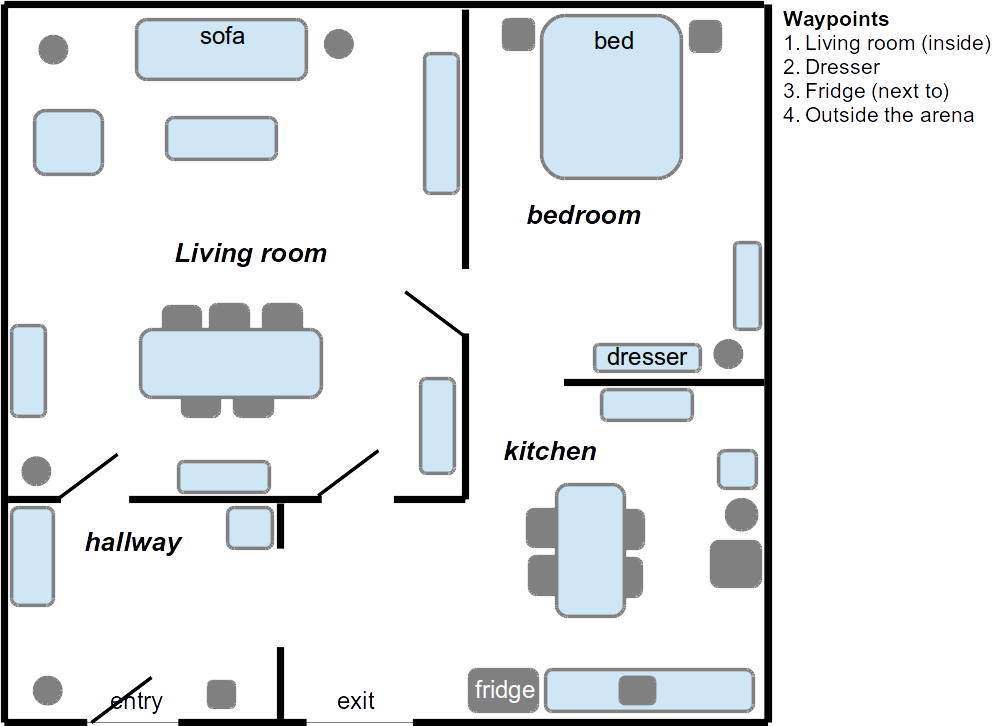
\includegraphics[width=0.5\columnwidth]{images/navigation.png}
	\caption{Navigation test: example setup.}
	\label{fig:restaurant}
\end{figure}

\paragraph*{Note 1:} Depending on the layout of the arena, waypoint 1 and 2 may be swapped.
\paragraph*{Note 2:} Reaching a waypoint means that the robot is looking at the waypoint-object and that the object is reachable by the robot's arm. 

\subsection{Obstacles}
While navigating to waypoints 1 and 2, the robot will find each of the following obstacles on its path:
\begin{itemize}
		\item \textbf{Small object:} Box sized object (between 5 and 15 cm per edge).  
		\item \textbf{3D Object:} A bar table, normal table, rolling chair: some object that is wider at its top than on its bottom, 
		  thus requiring more than just a laser scanner mounted near the ground to avoid obstacles.
		\item \textbf{Smart obstacle:} A person to whom the robot may speak to and kindly ask to move away. 
		  When interacting with people, the robot must look at the person and make clear is speaking with him/her.
	\end{itemize}

\subsection{Additional rules and remarks}
\begin{enumerate}
	\item \textbf{Show must go on:} If a robot is unable to reach a waypoint, it must say it and proceed to the next one.
	\item \textbf{Make it fast:} If a robot is absolutely unable to handle one or more obstacles, please inform the TC before the test so no time is wasted.
	\item \textbf{Closing doors:}  The door that will be shut will be the door on the route the robot has committed to. 
	  It will be shut right after the robot starts driving towards the door. 
	  The door will be closed well before the robot reaches it so the robot has enough time to notice that the door closed.	
	\item \textbf{Moving objects:} If the robot finds on its way a \textit{static movable obstacle} (chair, cubes, toys, etc.) which is capable to move, it may move the object apart with its manipulator.
	\item \textbf{When following people:} 
	\begin{enumerate}
		\item \textbf{Instruction:} The robot interacts with the operator, \emph{not} the team. That is, the team is not allowed to briefly instruct the operator.
		\item \textbf{Natural walking:} The operator has to walk \quotes{naturally}, i.e., move forward facing forward. 
		  The operator is not allowed to walk back, stand still, signal the robot or follow some re-calibration procedure.
		\item \textbf{Asking for passage:} The robot is allowed to (gently) ask people to step aside.
	\end{enumerate}
	
	\item \textbf{When guiding people:} 
	\begin{enumerate}
		\item \textbf{Instruction:} The robot interacts with the follower, \emph{not} the team. 
		  That is, the team is not allowed to briefly instruct the follower.
		\item \textbf{Asking for passage:} The robot is allowed to (gently) ask people to step aside.
	\end{enumerate}
\end{enumerate}

\subsection{Data recording}
  Please record the following data (See \refsec{rule:datarecording}):
  \begin{itemize}
   \item Mapping data
   \item Plans
  \end{itemize}

\subsection{Referee instructions}

The referee needs to
\begin{itemize}
	\item Instruct the OC and volunteers on when and where locate objects.
	\item Instruct the OC and volunteers on when and which doors must be closed.
	\item Stop the robot immediately when it is about to collide.
\end{itemize}

\subsection{OC instructions}

\textbf{2 hours before the test}
\begin{itemize}
	\item Announce the locations for waypoints 1, 2, and 3.
	\item Find a location for waypoint 4. 
\end{itemize}

\textbf{During the test}
\begin{itemize}
	\item Open and close the doors when instructed by the referee.
	\item Place the obstacles (or act as an obstacle) when instructed by the referee.
\end{itemize}

\newpage

\subsection{Score sheet}

The maximum time for this test is 5 minutes.

\begin{scorelist}

	\scoreheading{Waypoints}
	\scoreitem{10}{Reaching waypoint A}
	\scoreitem{10}{Reaching waypoint B}

	\scoreheading{Obstacles}
	\scoreitem{20}{Avoiding obstacle 1}
	\scoreitem{30}{Avoiding obstacle 2}
	\scoreitem{40}{Avoiding obstacle 3}
	\scoreitem{10}{Reporting unreachable waypoint due to an obstacle (will end the test)}

	\scoreheading{Doors}
	\scoreitem[2]{20}{Starting a new path after reaching a closed door}
	\scoreitem[2]{45}{Opening the door and continue instead of plan a new trajectory}

	\scoreheading{Optional tasks (up to 50 points)}
	\scoreitem{10}{Reaching waypoint}
	\scoreitem{40}{Reentering the arena after reach Waypoint 3}

	\setTotalScore{200}
\end{scorelist}


% Local Variables:
% TeX-master: "Rulebook"
% End:


% Local Variables:
% TeX-master: "Rulebook"
% End:
